% !TEX encoding   = UTF8
% !TEX spellcheck = ru_RU

\documentclass[a4paper,12pt,oneside,openany,final]{memoir}

\input{common/packages}
\input{common/biblatex}

\input{common/setup}
\input{setup}

\renewcommand*\paperSubject{\href{\latexurl}{\TeX}нические материалы семинаров}

\input{common/styles}
\input{styles}


\addbibresource{references.bib}




\begin{document}

%%==========================
\begin{pycode}
from sympy import *
\end{pycode}
%%==========================


\input{common/title}

\frontmatter
%%==========
\input{common/contents}

\include{intro}


\mainmatter
%%=========
\include{ch01/hello_world}
% !TEX encoding   = UTF8
% !TEX spellcheck = ru_RU
% !TEX root = ../seminars.tex

%%===========================
\chapter{Работа в \name{IDE}}\label{chap:ide}
%%===========================
В~ходе студенческой лабораторной работы по~физике получены данные измерений некоторой величины~\(y\), которая описывается линейной зависимостью \(y = a + bx\), где \(a\)~и \(b\) "--- какие-то константы. Полученные точки записаны в~файл, следуя простому формату:
\[
\begin{array}{ll}
    x_1 & y_1 \\
    x_2 & y_2 \\
    \vdots & \vdots \\
    x_N & y_N \\
\end{array}
\]
Количество пар координат не~указано и может быть произвольным. Несмотря на~линейную зависимость, точки не~ложатся строго на~прямую из-за различного рода погрешностей измерений.

Давайте напишем программу, которая считывает данные эксперимента из~файла и методом наименьших квадратов вычисляет коэффициенты \(a\) и \(b\), а также доверительные интервалы \(\pm\Delta a\) и \(\pm\Delta b\) соответственно.



%%==================================
\section{Метод наименьших квадратов}\label{sect:leastsquares}
%%==================================

%%===============================
\subparagraph{Постановка задачи.}
%%===============================
Рассмотрим регрессию (зависимость) следующего вида:
\begingroup
\newcommand{\SumN}{\ensuremath{\sum\limits_{i=1}^{N}}}
\begin{equation}\label{eq:linearmodel}
y_i = a + b x_i + \varepsilon_i,\quad i = \overline{1, N}.
\end{equation}
Среди всевозможных значений \(\{ a, b \}\) будем искать такие, которые приводят к~минимальной сумме квадратов отклонений (ошибок):
\[
S_{\varepsilon} = \SumN \varepsilon_i^2 = \SumN (y_i - a - b x_i)^2\quad\rightarrow\quad \min\limits_{a, b}.
\]
Запишем условие существования экстремума:
\[
\begin{array}{l}
    \dfrac{\partial}{\partial a} S_{\varepsilon} = -2 \SumN (y_i - a - b x_i) = 0, \\[2ex]
    \dfrac{\partial}{\partial b} S_{\varepsilon} = -2 \SumN (y_i - a - b x_i) x_i = 0, \\
\end{array}
\]
откуда получим систему линейных уравнений:
\[
\left\{ \begin{array}{l}
    \SumN y_i - N a - b\SumN x_i = 0, \\[2ex]
    \SumN x_i y_i - a\SumN x_i - b\SumN x_i^2 = 0. \\
\end{array} \right.
\]
Вводя обозначение для среднего арифметического множества значений некоторой величины \(f\):
\[
\bar f = \dfrac{1}{N}\SumN f_i,
\]
перепишем систему в~виде:
\[
\left\{ \begin{array}{l}
    \bar y - a - b\bar x = 0, \\
    \overline{x y} - a\bar x - b\overline{x^2} = 0, \\
\end{array} \right.
\]
и получим искомое решение:
\[
\boxed{ \begin{array}{l}
        a = \bar y - b\bar x, \\
        b = \dfrac{\overline{x y} - \bar x\bar y}{\overline{x^2} - \bar x^2}. \\
\end{array} }
\]
\endgroup



%%====================================
\subparagraph{Программная реализация.}
%%====================================
Решение этой задачи может быть выражено на~языке \lang{C++} следующим образом:\label{code:lsm}

\cppfile{projects/02/least_squares.cpp}



%%====================
\subparagraph{Сборка.}
%%====================
Чтобы собрать исполняемый файл из командной среды, или <<консоли>>, необходимо перейти в каталог с вашими проектами:

\console`$ cd /path/to/your/projects`

\noindent и вызвать \GCC:

\console`$ g++ -o bin/lsm -std=c++17 -pedantic -Wall -Wextra 02/least_squares.cpp`

\begin{figure}[h]
{\centering
    \hfill
    \subbottom[точки лежат строго на прямой\label{fig:lsm:a}]{%
        \includegraphics[width=0.45\textwidth]{images/line_exact.pdf}}
    \hfill
    \subbottom[точки не лежат на прямой\label{fig:lsm:b}]{%
        \includegraphics[width=0.45\textwidth]{images/line_approx.pdf}}
    \hfill
}
\caption{Линейная аппроксимация методом наименьших квадратов}
\label{fig:lsm}
\end{figure}



%%==========================
\subparagraph{Тестирование.}\label{test:lsm}
%%==========================
Полученная программа невелика, и, тем не менее, даже она может содержать приличное количество ошибок. Поэтому её работоспособность необходимо как следует проверить, запустив несколько разнообразных тестов. Приведём примеры:
\par\begin{itemfeature}
\item забыли указать имя файла:
\begin{consolecode}
$ bin/lsm
usage: bin/lsm  file_with_data
\end{consolecode}


\item файл не существует:
\begin{consolecode}
$ bin/lsm  not_exist.txt
error: can't open file 'not_exist.txt'
\end{consolecode}


\item файл пуст:
\begin{consolecode}
$ bin/lsm  02/empty.txt
error: division by zero
\end{consolecode}


\item идеальный случай (рис.\,\ref{fig:lsm:a}), когда точки лежат строго на прямой:
\begin{consolecode}
$ bin/lsm  02/line_exact.txt
line_exact.txt  0.25 0  0.88 0
\end{consolecode}


\item реальный случай (рис.\,\ref{fig:lsm:b}), когда точки лежат вдоль прямой с некоторым разбросом:
\begin{consolecode}
$ bin/lsm  02/line_approx.txt
line_approx.txt  0.262479 0  0.873039 0
\end{consolecode}
\end{itemfeature}



%%================
\WhatToReadSection
%%================
\textcite{Stroustrup:2016:ru}: \textbf{глава~4}



%%===============
\ExercisesSection
%%===============
\begin{exercise}
\item Доработайте программу, приведённую на странице~\pageref{code:lsm}. В функции \code{least\_squares} необходимо дополнительно вычислить доверительные интервалы.

Обязательно протестируйте вашу программу. Воспользуйтесь файлами, упомянутыми в подразделе на странице~\pageref{test:lsm}.


\item\hard\label{ex:plot} Продолжая предыдущее упражнение, напишите на \emph{любом} известном вам языке программу, которая рисует график, отражающий результаты лабораторной работы. На вход подаётся исходный файл с точками и оценки коэффициентов линейной регрессии.

Организуйте взаимодействие с программой из предыдущего упражнения так, чтобы можно было автоматически передавать входные данные. На выходе необходимо получить изображение на экране или в файле одного из популярных форматов, например \code{PNG}, с графиком, на котором маркерами нанесены экспериментальные точки, и сплошной линией "--- аппроксимирующая прямая.

Например, рисунок~\ref{fig:lsm} получен в результате выполнения этого упражнения с использованием языка \lang{Python}, пакета \name{Matplotlib} и командной среды (см. страницу~\pageref{sect:pyplot}).
\end{exercise}

\include{ch03/computation}
\include{ch04/errors}
\include{ch05/calculator_part_1}
\include{ch06/calculator_part_2}
% !TEX encoding   = UTF8
% !TEX spellcheck = ru_RU
% !TEX root = ../seminars.tex

%%============================================
\chapter{Технические детали: функции и прочее}
%%============================================

%%=====================================
\section{Система сборки \texttt{CMake}}
%%=====================================
В~прошлый раз для~сборки исполняемого файла программы <<калькулятор>> мы вызывали следующую команду:

\console`$ g++ -o bin/calc -Ilib -pedantic -Wall -Wextra 06/calculator.cpp`

Для~проектов с~более сложной структурой, состоящих из~множества файлов, подключающих внешние библиотеки, имеющих разные варианты конфигурации сборки, намного удобнее воспользоваться системой сборки, например, простым \name{Make}-ом или более мощным и переносимым между платформами \name{CMake}-ом.

По~сути, для~системы сборки мы тоже некоторым образом должны указать детали всей цепочки сборки проекта от~компилятора и его флагов до~исходных файлов с~кодом.



%%===================================
\paragraph{Установка \texttt{CMake}.}
%%===================================
Скачайте \href{\cmakeurl}{архив}\footnote{Дистрибутив CMake: \nolinkurl{\cmakeurl}} \code{CMake} и распакуйте его (например, рядом с~каталогом, куда был распакован \code{MinGW}). Добавьте путь к~папке \code{bin} в~системные пути поиска (переменная \code{PATH}, см.~страницу~\pageref{sect:winSetup}).

Для~поддержки \name{CMake}-а в~\name{VS\,Code} необходимо доставить плагин \textenglish{CMake Tools} от~компании Microsoft.

Поскольку данный плагин рассматривает рабочую директорию (\textenglish{workspace}) как единый проект, то необходимо создать корневой проект, который будет включать в~себя дочерние проекты. К~счастью, это не~сильно усложнит нашу задачу.

Корневой и дочерние проекты \name{CMake} должны называться одинаково \code{CMakeLists.txt}, отличаясь лишь положением в~файловой системе.



%%======================
\paragraph{Общий проект}
%%======================
необходимо разместить в~корне рабочей директории (у~нас это каталог \code{projects}). В~этот проект мы добавим общие настройки, такие как версия стандарта языка~\lang{C++} и дополнительные флаги компилятора (включим всевозможные предупреждения).

\cmakefile[firstline=3, lastline=5]{projects/CMakeLists.txt}

Далее, добавим в~стандартные пути каталог с~нашими библиотеками.

\cmakefile[firstline=7, lastline=11]{projects/CMakeLists.txt}

И, наконец, добавим наш первый дочерний проект, указав путь к~его директории. (Создайте указанный каталог для~проекта.)

\cmakefile[firstline=13, lastline=13]{projects/CMakeLists.txt}



%%================================
\paragraph{Проект <<калькулятор>>}\label{sect:calcproj}
%%================================
размещаем в~каталоге \code{projects/07/calculator}. Ещё раз повторим, что проектный файл создаётся один для~каждого каталога и поэтому на~всех уровнях вложения называется одинаково \code{CMakeLists.txt}. Эта идея наследуется от~\name{Make}.

Создадим локальную переменную \code{TARGET}. Она будет использоваться несколько раз. Поскольку удобно копировать проект для~других задач и заменять имя проекта только в~одном месте. Также это уменьшает вероятность появления ошибок.

\cmakefile[firstline=3, lastline=3]{projects/07/calculator/CMakeLists.txt}

Укажем имя проекта и язык программы (\lang{C++}). Для~получения значения локальной переменной используется знак \code{\$} и фигурные скобки: \code{\$\{TARGET\}}.

\cmakefile[firstline=9, lastline=9]{projects/07/calculator/CMakeLists.txt}

\noindent Добавим ещё одну локальную переменную \code{SOURCES} для~хранения списка файлов с~исходным кодом. (Если файлов несколько, просто перечисляем их через пробел или с~новой строки.)

\cmakefile[firstline=5, lastline=7]{projects/07/calculator/CMakeLists.txt}

\noindent Сообщим системе сборки, что нам нужен исполняемый файл с~именем \code{\$\{TARGET\}}, который состоит из~списка исходных файлов \code{\$\{SOURCES\}}.

\cmakefile[firstline=11, lastline=11]{projects/07/calculator/CMakeLists.txt}

В~завершение попросим систему сгенерировать инструкции для~установки исполняемого файла в~заданный каталог. Для~упрощения понимания, можно считать, что файл будет просто скопирован\footnote{В~действительности могут выполняться дополнительные действия (зависит от~платформы).}.

\cmakefile[firstline=13, lastline=13]{projects/07/calculator/CMakeLists.txt}



%%==========================================
\paragraph{Как назначить каталог установки?}
%%==========================================
В~настройки рабочей директории (\textenglish{Workspace Settings JSON}) необходимо добавить строку:

\jsonfile[firstline=5, lastline=5]{projects/.vscode/settings.json}

Чтобы выполнить установку, необходимо явно вызвать команду: \code{Ctrl+Shift+P} и в~строке поиска набрать \code{cmake\,install}.

Таким образом, исполняемый файл окажется в~каталоге \code{projects/bin}, как и ранее, когда мы непосредственно вызывали компилятор из~консоли.



%%================
\paragraph{P.\,S.}
%%================
Поиск компилятора, настройку флагов компиляции и массу другой работы \code{CMake} выполнит вместо нас в~процессе конфигурации. Этим процессом можно управлять. Однако, в~данный момент, нас вполне устроят базовые пресеты (\textenglish{Release, Debug}). Подробнее про систему сборки \code{CMake} можно почитать в~\href{\cmakedocurl}{документации}\footnote{Документация CMake: \nolinkurl{\cmakedocurl}}.



%%====================================
\section{Распределение кода по файлам}
%%====================================
Разместите логически отдельные части калькулятора в~разных файлах, опираясь на~материал \textbookref{главы~8}.

\begin{flushleft}\begin{tabular}{ll}
    \toprule
    \code{token.h}   & Лексемы и поток ввода лексем, константы \\
    \code{token.cpp} & \\[0.5em]

    \code{variable.h}   & Переменные и таблица переменных (символов) \\
    \code{variable.cpp} & \\[0.5em]

    \code{calculator.cpp} & Цикл вычислений, реализация грамматики \\
    \bottomrule
\end{tabular}\end{flushleft}

Помните, что заголовочные файлы должны содержать лишь объявления и константы, чтобы при~включении в~другие единицы трансляции не~происходило переопределение функций и глобальных переменных.

Как правило, содержимое заголовочного файла обрамляется директивами:

\begin{cppcode*}{linenos=false}
#ifndef TOKEN_H
#define TOKEN_H 1

// all code must be here

#endif // #ifndef TOKEN_H
\end{cppcode*}

\noindent Это необходимо во~избежание повторного включения кода из~файла \code{token.h} в~ту же единицу трансляции. (Когда и к~чему это может привести?) Такая ситуация неизбежно возникает в~любой достаточно большой программе.

Директива \cppinline/#ifndef/ проверяет определено ли имя \cppinline/TOKEN_H/. Если да, то она игнорирует весь код вплоть до~завершающей парной директивы \cppinline/#endif/. Если нет, тогда код включается, а \cppinline/TOKEN_H/ определяется при~помощи \cppinline/#define/, чтобы при~повторном подключении файла этот код пропускался. Имя макроса обычно формируют по~названию исходного заголовочного файла и набирают в~верхнем регистре.

Приведённый выше способ является наиболее переносимым между различными платформами. Некоторые компиляторы дополнительно поддерживают директиву, которая, по~сути, служит той же цели:

\cpp/#pragma once/



%%===========================
\section{Замена потока ввода}
%%===========================
Сделайте поток лексем явным параметром функций, как требуется в~упражнении~1 из~\textbookref{главы~8}. Например, функция \code{statement()} будет выглядеть так:

\begin{cppcode*}{linenos=false}
double statement (Token_stream& ts)
{
  Token t = ts.get();
  switch (t.kind)
  {
    case let:
      return declaration(ts);
    default:
      ts.putback(t);
      return expression(ts);
  }
}
\end{cppcode*}

\noindent Глобальную переменную \code{ts} можно (и нужно) сделать локальной:
\begin{cppcode*}{linenos=false}
void calculate ()
{
  Token_stream ts;

  while (true)
  try
  {
// as before

    out << result << statement(ts) << endl;
  }
  catch (runtime_error& e)
  {
// ...
    clean_up_mess(ts);
  }
}
\end{cppcode*}

Добавьте в~класс \code{Token\_stream} ссылку на~поток ввода и соответствующий конструктор для~инициализации. По~умолчанию, как и ранее, используйте стандартный поток ввода \code{cin}:

\begin{cppcode*}{linenos=false}
class Token_stream
{
  public:
  Token_stream() : in{ cin } {/* empty body */}
  Token_stream(istream& s) : in{ s } {/* empty body */}

// as before

  private:
// ...
  istream& in;
};
\end{cppcode*}

\noindent Определения методов класса следует поправить, заменив \code{cin} на~\code{in} или иное подходящее имя для~ссылки на~поток ввода.



%%================
\paragraph{P.\,S.}
%%================
После всех изменений, необходимо вновь прогнать тесты (см.~раздел на~странице~\pageref{sect:autotests}) и убедиться, что калькулятор остался в~рабочем состоянии.



%%==================================
\section{\texttt{constexpr} функции}
%%==================================
Немного дополним материл \textbookref{главы~8} по~данной теме\footcite[раздел 3.9]{Meyers:2016:ru}.

\begin{itemize}[itemindent=*, leftmargin=0pt]
    \item Функции, объявленные как \cppinline/constexpr/, могут использоваться в~контекстах, требующих константы времени компиляции. Если значения передаваемых вами аргументов в~\code{соnstехрr}-функцию в~таком контексте известны во~время компиляции, результат функции будет вычислен в~процессе компиляции. Если любое из~значений аргументов неизвестно во~время компиляции, ваш код будет отвергнут.

    \item Когда \code{соnstехрr}-функция вызывается с~одним или несколькими значениями, неизвестными во~время компиляции, она действует так же, как и обычная функция, выполняя вычисления во~время выполнения. Это означает, что вам не~нужны две функции для~выполнения одних и тех же операций, одной "--- для~констант времени компиляции, другой "--- для~всех прочих значений. Функция, объявленная как
    \code{constexpr}, выполняет их все.
\end{itemize}

Поскольку функции \code{constexpr} должны быть способны возвращать результаты во~время компиляции при~вызове со~значениями времени компиляции, на~их реализации накладываются ограничения. Эти ограничения различны в~\lang{C++11} и~\lang{C++14}.

В~\lang{C++11} функции \code{constexpr} могут содержать не~более одной выполнимой инструкции "--- \cppinline/return/. Это выглядит более ограничивающим, чем является на~самом деле, поскольку для~повышения выразительности \code{соnstехрr}-функций можно использовать две хитрости. Во-первых, можно применять условный оператор \code{"? :"} вместо инструкции \cppinline/if-else/, а во-вторых, вместо циклов можно использовать рекурсию. Таким образом, функция \code{pow} может быть реализована следующим образом:

\begin{cppcode*}{linenos=false}
constexpr int pow (int base, int exp) noexcept
{
  return exp == 0 ? 1 : base * pow(base, exp - 1);
}
\end{cppcode*}

Этот код работает, но только очень непритязательный функциональный программист сможет назвать его красивым. В~\lang{C++14} ограничения на~\code{constexpr}-функции существенно слабее, так что становится возможной следующая реализация:

\begin{cppcode*}{linenos=false}
constexpr int pow (int base, int exp) noexcept  // C++14
{
  auto res = 1;
  for (int i = 0; i < exp; ++i)
    res *= base;
  return res;
}
\end{cppcode*}



%%=====================================
\section{Сортировка пар (имя, возраст)}
%%=====================================
Приведём пример реализации программы из~упражнения~7 \textbookref{главы~8}. Будем придерживаться контекста исходного задания из~книги и использовать лишь изученные нами средства.

В~начале мы должны отсортировать вектор имён, а затем синхронизировать его с~вектором возрастов, используя копии исходных массивов.

\cppfile[firstline=48, lastline=56]{projects/07/name_age.cpp}

Чтобы синхронизировать пары, будем брать имена из~нового, сортированного, массива и искать их позицию в~старом массиве-копии. Взяв элемент из~старого массива возрастов с~той же позицией, мы получим парный элемент для~текущего имени.

\cppfile[firstline=28, lastline=46]{projects/07/name_age.cpp}

\noindent Отметим, что в~исходных данных может быть несколько пар с~одинаковыми именами. Мы сохраним их все, соблюдая тот порядок, в~котором они были исходно (\emph{стабильная сортировка}).

Вспомогательная функция поиска элемента в~массиве, начиная с~указанной позиции:

\cppfile[firstline=18, lastline=26]{projects/07/name_age.cpp}



%%==============================================
\paragraph{Функция \texttt{main} и ввод данных.}
%%==============================================
Тело \code{main} может выглядеть примерно таким образом:

\cppfile[firstline=81, lastline=81]{projects/07/name_age.cpp}
\cppfile[firstline=83, lastline=97]{projects/07/name_age.cpp}

Мы разместили каждое логическое действие в~отдельной функции. Самое сложное из~ещё не~рассмотренных нами действий "--- это ввод данных от~пользователя.

\cppfile[firstline=58, lastline=73]{projects/07/name_age.cpp}

Пары будут считываться, до~тех пор, пока мы не~завершим ввод при~помощи \code{Ctrl+D} в~\name{Linux} или \code{Ctrl+Z} в~\name{Windows}. Или пока не~введём некорректное значение для~возраста (почему для~возраста?), например, символ \code{'|'}. Появится ли некорректная пара в~последнем случае?

Вывод же на~печать пар имя/возраст теперь совсем не~составит труда.

\cppfile[firstline=75, lastline=79]{projects/07/name_age.cpp}



%%=======================
\paragraph{Тестирование.}
%%=======================
Воспользуйтесь перенаправлением ввода из~файла, чтобы протестировать полученную программу. Заготовьте пары в~отдельном файле \code{name\_age\_test\_in.txt}, и подайте их на~ввод программе, как это было показано в~предыдущем разделе на~странице~\pageref{par:inout}.



%%================
\paragraph{P.\,S.}
%%================
Слегка доработайте программу, улучшив приветствие пользователю и добавив <<штатное>> завершение ввода, например, по~команде \code{End}.



%%================
\WhatToReadSection
%%================
\textcite{Stroustrup:2016:ru}: \textbf{глава~9}



%%===============
\ExercisesSection
%%===============
\begin{exercise}
\item Выполните упражнения из~\textbookref{главы~8} учебника.

\end{exercise}

% !TEX encoding   = UTF8
% !TEX spellcheck = ru_RU
% !TEX root = ../seminars.tex

%%===========================================
\chapter{Технические детали: классы и прочее}
%%===========================================

%%====================================================
\section{Положение на плоскости. Класс \texttt{Vec2d}}
%%====================================================
Создадим небольшой вспомогательный класс \code{Vec2d} для~указания положения объекта на~плоскости. Позже мы сможем им воспользоваться при~рисовании двумерных фигур.

Заголовочный файл \code{lib/vec/vec2d.h} описывает данный класс, объявляет удобные операции над~его экземплярами.

\cppfile[firstline=4, lastline=13]{projects/lib/vec/vec2d.h}
\cpp`  // ...`
\cppfile[firstline=16, lastline=16]{projects/lib/vec/vec2d.h}
\cpp`// ...`
\cppfile[firstline=19, lastline=20]{projects/lib/vec/vec2d.h}
\cppfile[firstline=23, lastline=23]{projects/lib/vec/vec2d.h}

Загадочные имена параметров \code{lhs} и \code{rhs}, используемые при~перегрузке операторов, соответствуют сокращениям от~\textenglish{left hand side} (то есть слева от~оператора) и \textenglish{right hand side} (то есть справа от~оператора).

Реализацию методов разместим в~файле \code{lib/vec/vec2d.cpp}.

\cppfile[lastline=10]{projects/lib/vec/vec2d.cpp}
\cpp`// ...`
\cppfile[firstline=31, lastline=36]{projects/lib/vec/vec2d.cpp}
\cppfile[firstline=40, lastline=40]{projects/lib/vec/vec2d.cpp}

Добавьте остальные необходимые операторы самостоятельно.



%%=======================================
\section{Тесты для~класса \texttt{Vec2d}}
%%=======================================
Каким образом протестировать функционал нашего класса? Мы можем написать разнообразные выражения. Таким образом, мы охватим все возможные варианты его использования. На~этом этапе нас будет защищать сам компилятор, выдавая ошибки, если мы что-то не~реализовали или сделали это неправильным образом.

\begin{consolecode}
$ bin/vec
...
q + q      = {0, 2} [OK]
r + q      = {1, 1} [OK]
r += r     = {2, 0} [OK]
...
length(2 * s + 3 * p)     = 3.60555  [OK]
length(t)                 = 1.41421  [OK]
-----------
31 passed of 31 total
\end{consolecode}

Добавим файл \code{08/vec/main.cpp}. Сделаем набросок кода, чтобы получить вывод, подобный приведённому выше.

\cppfile[lastline=7]{projects/08/vec/main.cpp}
\cpp`// ...`
\cppfile[firstline=32, lastline=33]{projects/08/vec/main.cpp}
\cpp`  // ...`
\cppfile[firstline=55, lastline=66]{projects/08/vec/main.cpp}
\cpp`  // ...`
\cppfile[firstline=87, lastline=89]{projects/08/vec/main.cpp}

Тесты можно хранить в~векторе. Каждый элемент должен содержать выражение как строку (\code{std::string}), результат вычисления этого выражения (\code{Vec2d}) и ответ (\code{Vec2d}). Создадим для этого небольшую структуру.

\cppfile[firstline=9, lastline=14]{projects/08/vec/main.cpp}

Добавим реализацию операторов сравнения для~вектора на~плоскости, чтобы сравнивать результат с~ответом.

\cppfile[firstline=25, lastline=30]{projects/08/vec/main.cpp}

\noindent Нужно убедиться, что эти операторы верно запрограммированы, поскольку мы используем их для~проверки успешности прохождения тестов.

\cppfile[firstline=34, lastline=42]{projects/08/vec/main.cpp}

Добавим тесты, перебирая различные варианты, пытаясь <<сломать>> реализацию операций над~вектором \code{Vec2d}, найти выражения, которые могут не~сработать.

\cppfile[firstline=44, lastline=53]{projects/08/vec/main.cpp}

Каждый элемент вектора, имеющий тип \code{TestV}, мы инициализируем тройкой, например, \cppinline/{"r + r", r + r, {2, 0}}/. Однако, мы не~хотели бы дублировать выражение сначала в~строку, а затем как есть. По~этой причине мы добавили макрос, который получает такую пару из~обычного выражения (подобно тому, как это делали ранее, см.~страницу~\pageref{par:macro}).

\cppfile[firstline=23, lastline=23]{projects/08/vec/main.cpp}

По~аналогии, добавляем тесты для~функции \code{length()}.

\cppfile[firstline=68, lastline=85]{projects/08/vec/main.cpp}

К~сожалению, здесь мы не~можем использовать тип \code{TestV}. Нужно хранить не~пару векторов, а просто пару чисел. Для~этой цели придётся создать ещё один тип.

\cppfile[firstline=16, lastline=21]{projects/08/vec/main.cpp}

Далее мы познакомимся с~шаблонами, которые изящно решают эту проблему, подобно тому, как с~этой задачей справляется контейнер \code{std::vector}.



%%=================================
\section{Проект для \texttt{CMake}}
%%=================================
Скопируем проект, который создавали для~калькулятора (см.~страницу~\pageref{sect:calcproj}) и слегка подправим, изменив имя и список файлов с~исходным кодом (\code{08/vec/CMakeLists.txt}).

\cmakefile[firstline=3, lastline=11]{projects/08/vec/CMakeLists.txt}

Мы добавили переменную \code{HEADERS}, поскольку у~нас появился заголовочный файл. Соответственно, можно расширить список исходных файлов. Заголовки не~будут напрямую участвовать в~процессе компиляции, но среда разработки сможет узнать об~их существовании и отобразить в~проекте.

\cmakefile[firstline=15, lastline=15]{projects/08/vec/CMakeLists.txt}

\noindent Этот проект необходимо также добавить в~корневой проект (\code{projects/CMakeLists.txt}).

\cmakefile[firstline=15, lastline=15]{projects/CMakeLists.txt}



%%================================
\section{Элементы логических схем}
%%================================
Логические схемы полезны и применяются во~многих областях: от~создания простых электронно-вычислительных плат универсального назначения до~сложных схем управления различными устройствами, основными и вспомогательными системами разнообразной техники.

\begin{figure}[h]
    {\centering
        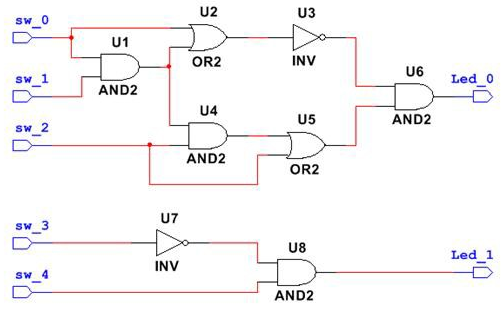
\includegraphics[width=0.6\textwidth]{images/logic_elements.png}

    }
    \caption{Пример рисования логической схемы}
    \label{fig:logicelems}
\end{figure}



%%========================
\paragraph{Анализ задачи.}
%%========================
Нам дан пример схемы с~логическими элементами. Нужно ответить на~следующие вопросы и сформулировать задачу.
\begin{enumerate}
    \item Какова предметная область?
    \begin{itemize}
        \item Работаем с~элементами математической логики.
    \end{itemize}

    \item В~каком контексте нужно разработать программный код?
    \begin{itemize}
        \item Необходим программный код, который позволяет смоделировать работу данной схемы.
        \item Этот код вполне вероятно будет использован для~моделирования подобных схем.
        \item Было бы удобно, если бы моделирование схемы не~зависело от~способа отображения процесса её работы (рисования).
    \end{itemize}

    \item Анализ исходных данных:
    \begin{itemize}
        \item На~схеме изображены не~все существующие логические элементы.
        \item На~схеме нет циклов.
        \item Вместо логического отрицания используются отрицания на~выходах/входах логических элементов.
    \end{itemize}
\end{enumerate}



%%=========================
\paragraph{Проектирование.}
%%=========================
Необходимо предусмотреть гибкость разрабатываемого программного кода.
\begin{itemize}
    \item Расширение функционала не~должно вынуждать полностью переписывать исходный код.
    \item Разделение на~небольшие части, подзадачи, которые могут быть использованы независимо (принцип <<разделяй и властвуй>>).
    \item Необходимо предусмотреть наиболее удобные уровни абстракции.
\end{itemize}

\bigskip Выделим в~коде две части:
\begin{itemize}
    \item Код для~непосредственного моделирования работы схемы.
    \item Код для~отображения процесса работы схемы (рисование).
\end{itemize}

\bigskip Продумаем примеры того, как бы мы хотели видеть использование разработанного программного кода:
\begin{enumerate}
    \item Создание элементов.
    \begin{itemize}
        \item При~создании логического элемента нужно указать его тип (тип объекта), инвертирован ли его выход (по~умолчанию не~инвертирован), задать \code{callback}-функцию (по~умолчанию \code{nullptr}).
        \item При~создании источника логического значения (сигнала) нужно указать это значение (по~умолчанию \code{false})
    \end{itemize}

    \item Соединение элементов.
    \begin{itemize}
        \item Соединений между логическими элементами гораздо больше, чем самих элементов.
        \item При~попытке сделать цикл в~схеме должно генерироваться исключение.
        \item Нужно предусмотреть (насколько это возможно) интуитивно понятный и лаконичный способ для~задания соединений.
        \item Удобно было бы соединять элементы по~цепочке.
        \item Будем использовать оператор \code{>>} для~соединения элементов (\code{and1 >> or2}).
        \item Подключение на~инвертированный вход вполне удобно смотрится с~использованием оператора~\code{\textasciitilde} (\code{or3 >> \textasciitilde{}and5}).
    \end{itemize}

    \item Изменение элементов.
    \begin{itemize}
        \item Для~задания логического значения источника удобно использовать оператор~\code{=}.
        \item Расчёт значений на~выходе каждого логического элемента должно происходить автоматически при~изменении состояния на~выходе элементов ниже по~цепочке.
        \item При~изменении состояния на~выходе элемента, этот элемент должен вызывать \code{callback}-функцию.
    \end{itemize}

    \item Получение значения на~выходе логического элемента.
    \begin{itemize}
        \item Оператор преобразования логического элемента в~значение \code{bool}.
    \end{itemize}

    \item Программный код для~отображения схемы и процесса её работы.
    \begin{itemize}
        \item Над этими деталями мы поразмышляем позднее.
    \end{itemize}
\end{enumerate}



%%============================
\paragraph{Первая реализация.}\label{par:logic:v1}
%%============================
Предлагаем самостоятельно разработать первую версию на~основе материала \textbookref{главы~9}.



%%================
\paragraph{P.\,S.}
%%================
Позже мы вернёмся к~проектированию классов для~моделирования схемы логических элементов, когда познакомимся с~наследованием и основами объектно-ориентированного программирования. Также мы добавим отрисовку элементов на~экране.



%%================
\WhatToReadSection
%%================
\textcite{Stroustrup:2016:ru}: \textbf{глава~10}



%%===============
\ExercisesSection
%%===============
\begin{exercise}
\item Выполните упражнения из~\textbookref{главы 9} учебника.

\end{exercise}

\include{ch09/io_streams}
\include{ch10/customizing_io}
% !TEX encoding   = UTF8
% !TEX spellcheck = ru_RU
% !TEX root = ../seminars.tex

%%==============================
\chapter{Модель вывода на экран}
%%==============================

%%=======================================
\section{Сборка библиотеки \texttt{FLTK}}
%%=======================================
\todo{\ldots добавить описание\ldots}



%%=============================
\section{Графические примитивы}
%%=============================
Рассмотрим пример из~\textbookref{раздела~12.7}, использующий графические классы.

\begin{figure}[ht]
    {\centering
        \includegraphics[width=0.6\textwidth]{images/shapes.png}

    }
    \caption{Окно программы c~графическими примитивами из~\textbookref{раздела~12.7}}
\end{figure}

\noindent Исходные файлы и проект программы размещены в~\href{\courserepourl}{репозитории}.

\begin{center}
    \code{projects/ch12/shape\_primitives}
\end{center}



%%=============
\paragraph{NB!}
%%=============
Использование директивы \code{using} приводит к~конфликту имён. В~системных графических библиотеках \name{Windows} определена функция \code{Rectangle}, а в~нашей графической библиотеке определён класс с~таким же именем. В~результате, компилятор обнаруживает неоднозначность определения имени.

Тем не~менее, поскольку все наши типы и функции размещены в~отдельном пространстве имён, следует просто уточнить, что мы имеем в~виду класс \code{Graph\_lib::Rectangle}.

\cppfile[firstline=1, lastline=10]{projects/ch12/shape_primitives/main.cpp}
\cppfile[firstline=12, lastline=21]{projects/ch12/shape_primitives/main.cpp}
\cpp`// ...`
\cppfile[firstline=48, lastline=51]{projects/ch12/shape_primitives/main.cpp}
\cpp`// ...`
\cppfile[firstline=113, lastline=113]{projects/ch12/shape_primitives/main.cpp}



%%=================================================
\section{Включение библиотеки \name{FLTK} в~проект}
%%=================================================
Рассмотрим внутренности проектного файла \code{CMakeLists.txt}, связанные с~добавлением внешней зависимости.

В~проект необходимо добавить файлы из~библиотеки \code{Graph\_lib}, которые будут подробно рассмотрены в~последующих \textbookref{главах} учебника. Классы этой библиотеки предоставляют нам сравнительно небольшой набор графических возможностей, реализованных на~основе библиотеки \name{FLTK}.

\cmakefile[firstline=5, lastline=5]{projects/ch12/shape_primitives/CMakeLists.txt}
\cmake'    # ... (our headers)'
\cmakefile[firstline=6, lastline=13]{projects/ch12/shape_primitives/CMakeLists.txt}
\cmake'    # ... (our sources)'
\cmakefile[firstline=15, lastline=18]{projects/ch12/shape_primitives/CMakeLists.txt}

Система сборки \name{CMake} имеет механизмы поиска <<внешних>> библиотек в~системе. Это позволяет уменьшить зависимость описания проекта от~платформы, оставляя при~этом возможность вручную задать конкретные пути к~ним в~процессе конфигурации. Для поиска библиотеки \name{FLTK}, а также её зависимости "--- библиотеки более низкого уровня \name{OpenGL}, нужно добавить следующие строки:

\cmakefile[firstline=25, lastline=26]{projects/ch12/shape_primitives/CMakeLists.txt}

\noindent Флаг \code{REQUIRED} указывает, что без~данного компонента невозможна успешная сборка проекта. Таким образом, мы получаем более раннюю диагностику в~виде ошибки на~этапе конфигурирования.

\todo{\ldots добавить дальнейшее описание\ldots}



%%================
\paragraph{P.\,S.}
%%================
Подводя итоги, перечислим необходимые в проекте компоненты для сборки программы, которая использует сторонние библиотеки:
\begin{itemfeature}
    \item пути к заголовкам;
    \item пути к библиотекам;
    \item дополнительные флаги компилятору;
    \item библиотеки;
    \item дополнительные флаги компоновщику.
\end{itemfeature}
Эти возможности присутствуют в каждой более-менее приличной среде разработки. Однако способы их добавления зависят от конкретной среды и могут сильно отличаться. Необходимо изучать соответствующие руководства.



%%========================================================
\paragraph{Сборка в \name{Unix}-подобной командной среде.}
%%========================================================
Библиотека \name{FLTK} предоставляет удобную утилиту \code{fltk-config}, с помощью которой можно узнать необходимые настройки для сборки проекта, например:

\begin{consolecode}
$ fltk-config --cxxflags
-I/usr/local/include -I/usr/include/freetype2 -I/usr/include/libpng16 \
-D_LARGEFILE_SOURCE -D_LARGEFILE64_SOURCE -D_THREAD_SAFE -D_REENTRANT
$ fltk-config --ldflags
-L/usr/local/lib -lfltk -lXrender -lXcursor -lXfixes -lXext -lXft \
-lfontconfig -lXinerama -lpthread -ldl -lm -lX11
\end{consolecode}

\noindent и собрать исполняемый модуль программы:

\begin{consolecode}
$ g++ -o bin/shapes -std=c++14 -pedantic $(fltk-config --cxxflags) \
  projects/ch12/shape_primitives/main.cpp lib/Graph_lib/*.cpp \
  $(fltk-config --use-images --ldflags)
\end{consolecode}

Обратите внимание на использование конструкции \code{\$(command)} "--- аналог косых кавычек \code{`command`}. Командная среда вначале выполняет команду \code{command}, а затем подставляет на её место результат (то, что вывелось бы на экран) и запускает образовавшуюся в итоге команду.

Стандартный способ узнать возможности какой-либо утилиты "--- вызвать справку:
\console`$ fltk-config --help`%$

Теперь можно запустить нашу программу:
\console`$ bin/shapes`%$



%%==========================
\section{Элементы геометрии}\label{sect:geomelems}
%%==========================
Напишем ряд вспомогательных функций. Чтобы не загромождать основную программу и в дальнейшем иметь возможность использовать код повторно, разместим их в отдельном модуле (\code{lib/poly}): \code{poly.h}/\code{poly.cpp}.

Функция \code{regular\_polygon()} возвращает список вершин правильного \code{n}-угольника с центром в точке \code{center}, радиусом описанной окружности \code{radius} и начальным положением (углом) \code{angle} первой вершины, отсчитывая от оси X. Последний параметр позволяет задать необходимую ориентацию на плоскости нашего многоугольника. Положительное значение угла задаёт вращение против часовой стрелки. По умолчанию значение этого угла равно \code{0}.

\cppfile[firstline=17, lastline=32]{projects/lib/poly/poly.cpp}

Изменение координат точки при вращении можно выразить через поворот самой системы координат:

\noindent
\parbox[c]{0.65\textwidth}{%
\[
  \left\{ \begin{array}{l}
    x = x\prime\cos\alpha - y\prime\sin\alpha, \\
    y = x\prime\sin\alpha + y\prime\cos\alpha.
  \end{array}\right.
\]
Используя эти соотношения, функция \code{rotated()} выполняет поворот точки \code{point} на угол \code{angle} относительно центра вращения \code{center} (положительный угол отмеряется против часовой стрелки) и возвращает новую точку. По умолчанию центр вращения расположен в начале координат.
}\hfill\parbox[c]{0.35\textwidth}{%
\begin{center}\begin{tikzpicture}[>=Stealth, very thick]
  \draw[help lines, step=.5cm] (-2, -1) grid (2.5, 2.5);
  \draw[->] (-0.5, 0) -- (2, 0) node[at end, below=3pt, fill=white] {\(x\)};
  \draw[->] (0, -0.5) -- (0, 2) node[at end, right=3pt, fill=white] {\(y\)};
  \draw[->, blue] (1.5, 0) arc [start angle=0, end angle=30, radius=1.5cm] node[midway, right=2pt, color=blue, fill=white] {\(\alpha\)};
  \draw[->, blue, rotate=30] (-0.5, 0) -- (2, 0) node[at end, above=1pt, color=blue, fill=white] {\(x\prime\)};
  \draw[->, blue, rotate=30] (0, -0.5) -- (0, 2) node[at end, left=1pt, color=blue, fill=white] {\(y\prime\)};
\end{tikzpicture}\end{center}
}% parbox

\cppfile[firstline=7, lastline=15]{projects/lib/poly/poly.cpp}

Функция \code{lerp()} добавлена в стандартную библиотеку \lang{C++20}. Она выполняет линейную интерполяцию между \(a\) и \(b\) для параметра \(t\) (или экстраполяцию, если \(t \notin [0, 1]\)).

\cppfile[firstline=30, lastline=30]{projects/lib/poly/poly.h}

Будет удобна ещё одна простая функция \code{append()}, которая добавит точки из списка в замкнутую ломаную \code{Closed\_polyline} из нашей графической библиотеки.

\cppfile[firstline=34, lastline=38]{projects/lib/poly/poly.cpp}

\noindent Здесь функция \code{as\_point()} преобразует вещественный радиус-вектор \code{Vec2d} в экранную точку \code{Point}, выполняя округление до целых значений по правилам математики.

\cppfile[firstline=32, lastline=35]{projects/lib/poly/poly.h}

\noindent Такое округление улучшает точность отрисовки линий на экране.



%%================
\section{Фракталы}
%%================
\emph{Фракталом} называется структура, состоящая из частей, которые в каком-то смысле подобны целому. Этот существенный отличительный признак наблюдается в эксперименте: фрактал выглядит одинаково, в каком бы масштабе его ни наблюдать. Взять хотя бы некоторые прекрасные кучевые облака. Они состоят из огромных <<горбов>>, на которых возвышаются <<горбы>> поменьше, на тех "--- <<горбы>> ещё меньше и т.д. вплоть до самого малого масштаба, который вы в состоянии разрешить.

\begin{figure}[ht]
    {\centering
        \includegraphics[height=0.26\textwidth]{images/fern.jpg}\hfil
        \includegraphics[height=0.26\textwidth]{images/clouds.jpg}\hfil
        \includegraphics[height=0.26\textwidth]{images/romanesco_broccoli.jpg}

    }
    \caption{Примеры фракталов в природе}
\end{figure}



%%========================
\paragraph{Снежинка Коха,}
%%========================
построенная в виде замкнутой кривой на базе равностороннего треугольника, впервые была описана шведским математиком \href{https://ru.wikipedia.org/wiki/Кох,_Нильс_Фабиан_Хельге_фон}{Хельге фон Кохом} в 1904 году. В некоторых работах она получила название «остров Коха».

Доказано, что эта фрактальная кривая обладает рядом любопытных свойств. К примеру, длина её периметра равна бесконечности, что, однако, не мешает охватывать конечную площадь, величина которой равна \(\frac{8}{5}\) площади базового треугольника.

\begin{figure}[ht]
    {\centering
        \includegraphics[width=0.3\textwidth]{images/koch_snowflake_n=0.png}\hfil
        \includegraphics[width=0.3\textwidth]{images/koch_snowflake_n=1.png}\hfil
        \includegraphics[width=0.3\textwidth]{images/koch_snowflake_n=5.png}

    }
    \caption{Снежинка Коха}
    \label{fig:kochshowflake}
\end{figure}

Построение кривой Коха начинается с прямолинейного отрезка единичной длины. Этот исходный отрезок называется \emph{затравкой} и может быть заменён каким-нибудь многоугольником, например, равносторонним треугольником или квадратом. Затравка "--- это \(0\)-е поколение кривой Коха. Далее, каждое звено затравки заменяется \emph{образующим элементом} "--- отрезок делится на 3 равные части и средняя часть заменяется равносторонним треугольником, у которого удалено основание (рисунок~\ref{fig:kochshowflake}).

Шаг этого алгоритма можно выразить следующим образом, используя ранее приведённые вспомогательные функции:

\cppfile[firstline=24, lastline=37]{projects/ch12/koch_snowflake/main.cpp}

Контейнер \code{std::list} представляет собой двусвязный список. Обойти его элементы можно используя итераторы "--- обобщённый аналог указателей. Они будут рассмотрены в \textbookref{главе~20} учебника.

Вариант рисования снежинки Коха на базе правильного \code{n}-угольника в окне шириной~\code{w} средствами нашей библиотеки \code{Graph\_lib} можно записать так:

\cppfile[firstline=51, lastline=80]{projects/ch12/koch_snowflake/main.cpp}

Мы добавили текстовую метку в центре фигуры, показывающую номер шага алгоритма. И также учли, что дальнейшее измельчение кривой бессмысленно, если длина ребра становится менее~\(1\) пикселя. Функцию \code{max\_edge\_length()} предлагаем реализовать самостоятельно.

\textbf{NB!} Обратите особое внимание, что замкнутая ломаная создаётся в теле цикла каждый раз заново. Дело в том, что \code{Graph\_lib} не предоставляет удобного способа добавления новых точек в середину кривой. Мы вынуждены откреплять нашу кривую от окна в конце итерации, чтобы избежать отрисовки несуществующего объекта.


%=================
\input{ch12/extra}
%=================



%%================
\WhatToReadSection
%%================
\textcite{Stroustrup:2016:ru}: \textbf{глава~13}



%%===============
\ExercisesSection
%%===============
\begin{exercise}
\item Выполните упражнения из \textbookref{главы~12} учебника.

\item Постройте так называемую антиснежинку Коха. Алгоритм генерирования заключается в вырезании на каждом этапе всё новых и новых треугольников из исходного многоугольника. Иными словами, рёбра базовой формы модифицируются внутрь, а не наружу. В результате полученная фигура охватывает бесконечное множество несвязанных областей.

\begin{figure}[ht]
  {\centering
    \includegraphics[height=0.2\textwidth]{images/koch_curve_85_degrees.png}

  }
  \caption{Фрактал Цезаро "--- вариант кривой Коха с углом между \(60^{\circ}\) и \(90^{\circ}\) (\(85^{\circ}\))}
\end{figure}

\item Нарисуйте дракона Хартера, также известного как дракона Хартера--Хейтуэя. Он был впервые исследован физиками \name{NASA} "--- Джоном Хейтуэем (John Heighway), Брюсом Бэнксом (Bruce Banks), и Вильямом Хартером (William Harter). В 1967 году описан Мартином Гарднером в колонке «Математические игры» журнала <<\textenglish{Scientific American}>>. Многие из свойств фрактала были описаны Чендлером Дэвисом (Chandler Davis) и Дональдом Кнутом.

\begin{figure}[ht]
  \begin{center}
    \fbox{\begin{minipage}{0.4\textwidth}
      \includegraphics[width=\textwidth]{images/harter-heighway_dragon_steps-1.jpg}\\
      \includegraphics[width=\textwidth]{images/harter-heighway_dragon_steps-2.png}
    \end{minipage}}
    \hfil
    \fbox{\begin{minipage}{0.25\textwidth}
      \includegraphics[width=\textwidth]{images/harter-heighway_dragon.png}
    \end{minipage}}
  \end{center}
  \caption{Дракон Хартера--Хейтуэя}
\end{figure}

\end{exercise}

\include{ch13/graphics_classes}
% !TEX encoding   = UTF8
% !TEX spellcheck = ru_RU
% !TEX root = ../seminars.tex

%%==========================================
\chapter{Проектирование графических классов}
%%==========================================

%%===========================================
\section{Элементы логических схем (версия 2)}
%%===========================================
Ранее мы рассматривали вопросы проектирования классов для~моделирования работы логических схем (см. страницу~\pageref{logic:elemfirst}). Однако тогда мы ещё не~были знакомы с~наследованием, поэтому при~реализации на~практике остались моменты, которые мы бы хотели пересмотреть и улучшить.

\begin{figure}[h]
  {\centering
    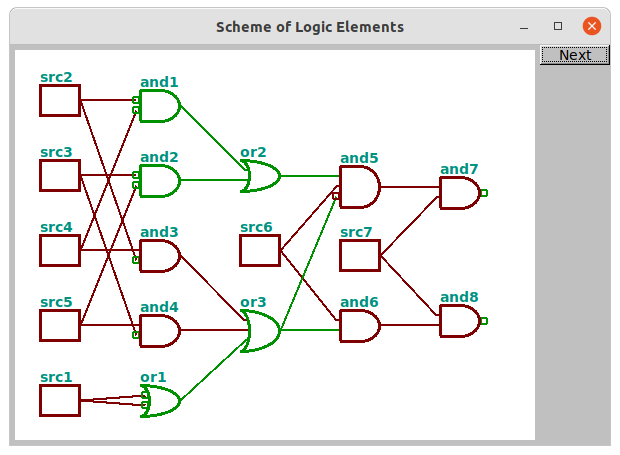
\includegraphics[width=0.6\textwidth]{images/logic_shapes.png}

  }
  \caption{Пример рисования логической схемы}
  \label{fig:logicshapes}
\end{figure}

Попробуем проанализировать задачу и продумать вопросы проектирования ещё раз, учитывая полученный опыт.



%%========================
\paragraph{Анализ задачи.}
%%========================
Нам дан пример схемы с~логическими элементами. Нужно ответить на~следующие вопросы и сформулировать задачу.
\begin{enumerate}
  \item Какова предметная область?
  \begin{itemize}
      \item Работаем с~элементами математической логики.
  \end{itemize}

  \item В~каком контексте нужно разработать программный код?
  \begin{itemize}
    \item Необходим программный код, который позволяет смоделировать работу данной схемы.
    \item Этот код вполне вероятно будет использован для~моделирования подобных схем.
    \item Было бы удобно, если бы моделирование схемы не~зависело от~способа отображения процесса её работы (рисования).
  \end{itemize}

  \item Анализ исходных данных:
  \begin{itemize}
    \item На~схеме изображены не~все существующие логические элементы.
    \item На~схеме нет циклов.
    \item Вместо логического отрицания используются отрицания на~выходах/входах логических элементов.
  \end{itemize}
\end{enumerate}



%%=========================
\paragraph{Проектирование.}
%%=========================
Необходимо предусмотреть гибкость разрабатываемого программного кода.
\begin{itemize}
  \item Расширение функционала не~должно вынуждать полностью переписывать исходный код.
  \item Разделение на~небольшие части, подзадачи, которые могут быть использованы независимо (принцип <<разделяй и властвуй>>).
  \item Необходимо предусмотреть наиболее удобные уровни абстракции.
\end{itemize}

\bigskip Выделим в~коде две части:
\begin{itemize}
  \item Код для~непосредственного моделирования работы схемы.
  \item Код для~отображения процесса работы схемы (рисование).
\end{itemize}

\bigskip Продумаем примеры того, как бы мы хотели видеть использование разработанного программного кода:
\begin{enumerate}
  \item Создание элементов.
  \begin{itemize}
    \item При~создании логического элемента нужно указать его тип (тип объекта), инвертирован ли его выход (по~умолчанию не~инвертирован), задать \code{callback}-функцию (по~умолчанию \code{nullptr}).
    \item При~создании источника логического значения (сигнала) нужно указать это значение (по~умолчанию \code{Signal::off}).
  \end{itemize}

  \item Соединение элементов.
  \begin{itemize}
    \item Соединений между логическими элементами гораздо больше, чем самих элементов.
    \item При~попытке сделать цикл в~схеме должно генерироваться исключение.
    \item Нужно предусмотреть (насколько это возможно) интуитивно понятный и лаконичный способ для~задания соединений.
    \item Удобно было бы соединять элементы по~цепочке.
    \item Будем использовать оператор~\code{>>} для~соединения элементов (\code{and1 >> or2}).
    \item Подключение на инвертированный вход вполне удобно смотрится с использованием оператора \code{\textasciitilde} (\code{or3 >> \textasciitilde{}and5}).
  \end{itemize}

  \item Изменение элементов.
  \begin{itemize}
    \item Для~задания логического значения источника удобно использовать оператор~\code{=} (\code{src1 = Signal::on}).
    \item Расчёт значений на~выходе каждого логического элемента должно происходить автоматически при~изменении состояния на~выходе элементов ниже по~цепочке.
    \item При~изменении состояния на~выходе элемента, этот элемент должен вызывать \code{callback}-функцию.
  \end{itemize}

  \item Получение значения на~выходе логического элемента.
  \begin{itemize}
    \item Оператор преобразования логического элемента в~значение \code{bool}.
  \end{itemize}

  \item Программный код для~отображения схемы и процесса её работы.
  \begin{enumerate}
    \item Нужно задавать только объекты, которые соответствуют логическим элементам на~схеме.
    \item Удобно создать класс-хранилище графических объектов \code{SchemeShape}.
    \item Отображение связей будет автоматическое, генерация объектов будет происходить в~\code{SchemeShape}.
    \item При~создании графических объектов нужно указать:
    \begin{itemize}
      \item на~какой схеме они расположены;
      \item какой логический элемент представляют;
      \item подпись (имя элемента);
      \item положение на~схеме.
    \end{itemize}
    \item Объект графического представления будет задавать \code{callback}-функцию для~элемента, который представляет.
    \item В~\code{callback}-функции будет происходить изменение цвета отображения элемента и связей.
  \end{enumerate}
\end{enumerate}



%%===================================
\section{Разработка логической части}
%%===================================
%%=========================================
\paragraph{Диаграмма наследования классов.}
%%=========================================
Набросаем иерархию классов, которые будут отражать наше представление о~логических элементах и взаимосвязях между ними.

\begin{center}\begin{tikzpicture}[node font=\ttfamily\small, >=Stealth]
    \graph [layered layout, components go right top aligned, edge=<-]
    {
        Scheme[text=blue];

        Element[align here, text=blue] ->[blue] {
            Source[text=blue],
            Operation[text=blue]
        };
        Operation ->[blue] {
            And[text=blue],
            Or[text=blue]
        };
    };

    \begin{scope}[on background layer]
        \node (Logic) [draw, blue, dashed, rounded corners,
        fit=(Element) (Source) (Scheme) (Operation) (And) (Or)] {};
        \node[text=blue, inner sep=0pt, above left=0pt of Logic.north west] {Logic};
    \end{scope}
\end{tikzpicture}\end{center}


%%=====================
\paragraph{Реализация.}
%%=====================
Объявление классов разместим в заголовочном файле \code{logic.h}, а реализацию методов и вспомогательных функций "--- в файле \code{logic.cpp}.

\bigskip
\todo{Ключевые моменты реализации будут размещены позднее.}


\clearpage
%%====================================
\section{Разработка графической части}
%%====================================
%%=========================================
\paragraph{Диаграмма наследования классов.}
%%=========================================
Для~графического изображения логических элементов нам придётся создать схожую иерархию классов. Отметим, что мы намерены отделить логику работы схем от~их рисования на~экране. Очевидно, мы могли бы отобразить нашу схему различными способами. Например, вывести структуру и состояние схемы в~консоль, нарисовать элементы с помощью графической библиотеки, и, наконец, сгенерировать файл с~описанием схемы для таких систем визуализации графов, как \name{GraphViz} или пакета \name{Tikz} системы вёрстки \LaTeX.

\begin{center}\begin{tikzpicture}[node font=\ttfamily\small, >=Stealth]
    \graph [layered layout, components go right top aligned, edge=<-]
    {
        Scheme[text=gray];

        Element[align here, text=gray, left=0pt] ->[gray] {
            Source[text=gray],
            Operation[text=gray]
        };
        Operation ->[gray] {
            And[text=gray],
            Or[text=gray]
        };

        Shape[as=Graph\_lib::Shape] -> ElementShape[text=blue] ->[blue] {
            SourceShape[text=blue],
            OperationShape[text=blue]
        };
        OperationShape ->[blue] {
            AndShape[text=blue],
            OrShape[text=blue]
        };
        Shape -> Rectangle[as=Graph\_lib::Rectangle] -> SchemeShape[text=blue];

        Element ->[edge=--, gray, dashed] ElementShape;

        { [same layer] Scheme, Element, ElementShape, SchemeShape };
    };

    \begin{scope}[on background layer]
        \node (Logic) [draw, gray, dashed, rounded corners, fit=(Element) (Source) (Scheme) (Operation) (And) (Or)] {};
        \node[text=gray, inner sep=0pt, above left=0pt of Logic.north west] {Logic};

        \node (GraphLib) [fit=(Shape) (Rectangle)] {};
        \node (ShapeLogic) [draw, blue, dashed, rounded corners, fit=(ElementShape) (SourceShape) (SchemeShape) (OperationShape) (AndShape) (OrShape)] {};
        \node[text=blue, inner sep=0pt, above right=0pt of ShapeLogic.north east] {Logic};
    \end{scope}
\end{tikzpicture}\end{center}



%%=====================
\paragraph{Реализация.}
%%=====================
Объявление графических классов и констант для управления стилем разместим в заголовочном файле \code{logic\_shapes.h}, а реализацию методов и вспомогательных функций "--- в файле \code{logic\_shapes.cpp}.

\bigskip
\todo{Ключевые моменты реализации будут размещены позднее.}



%%================
\WhatToReadSection
%%================
\textcite{Stroustrup:2016:ru}: \textbf{глава~15}



%%===============
\ExercisesSection
%%===============
\begin{exercise}
\item Выполните упражнения из \textbookref{главы~14} учебника.

\end{exercise}

% !TEX encoding   = UTF8
% !TEX spellcheck = ru_RU
% !TEX root = ../seminars.tex

%%==================================================
\chapter{Графическое представление функций и данных}
%%==================================================

%%==========================================
\section{Улучшение класса \texttt{Function}}
%%==========================================
Представим вариант выполнения упражения~2 из~\textbookref{главы~15}.

\cppfile[firstline=11, lastline=29]{projects/ch15/function.cpp}

Первый раз основную работу по~вычислению и сохранению точек выполняет конструктор базового класса \code{Function}. Нам остаётся сохранить параметры, задающие вид кривой:

\cppfile[firstline=31, lastline=36]{projects/ch15/function.cpp}

Метод \code{move()} перекрывает \code{Shape::move()}, чтобы сдвинуть начало координат для~правильного вычисления точек кривой, если будут внесены какие-либо дополнительные изменения (форма кривой, диапазон рисования, и т.\,д.):

\cppfile[firstline=38, lastline=43]{projects/ch15/function.cpp}

Следующие функции позволяют пользователю изменить вид кривой:

\cppfile[firstline=45, lastline=64]{projects/ch15/function.cpp}

Основную работу при~этом выполняет закрытая функция \code{redistribute()}, которая вычисляет точки кривой заново:

\cppfile[firstline=66, lastline=75]{projects/ch15/function.cpp}

Заметим, что хранение точек в~классе \code{Shape} (подобно тому, как это делает \code{Graph\_}\-\code{lib::Function}) не~позволяет нам уменьшить их количество. По~этой причине мы не~предоставляем пользователю возможность изменять число точек.

Как и всегда, необходимо протестировать новые возможности, например, так:

\cppfile[firstline=116, lastline=133]{projects/ch15/function.cpp}



%%===================
% !TEX encoding   = UTF8
% !TEX spellcheck = ru_RU
% !TEX root = ../seminars.tex

%%====================================
\section{Функторы или объекты-функции}
%%====================================
Эта тема уже была затронута в~разделе на~странице~\pageref{sect:lambda} в~связи с~обсуждением лямбда-выражений. Кратко вспомним этот материал ещё раз и применим его для~решения небольшой задачки.

\emph{Функтором} называют объекты некоторого класса, в~котором перегружен оператор вызова \code{operator()}. Использование этого оператора синтаксически выглядит как вызов обычной функции. Таким образом, там, где синтаксически требуется вызов функции, можно использовать как простые функции, так и объекты-функции. Например, в~алгоритмах стандартной библиотеки языка~\lang{C++}.

Важные отличия объекта-функции от~обычной функции:
\begin{itemfeature}
  \item можно хранить некоторое состояние и извлекать его после вызова;
  \item количество аргументов можно уменьшить (за~счёт хранения ссылок и данных внутри объекта);
  \item эффективность: часто код функции \code{operator()} короткий и размещается внутри класса. Компилятор делает его подставляемым (\code{inline}). Это редко бывает возможным при~вызове обычной функции через указатель.
\end{itemfeature}



%%==============================================================
\paragraph{Вычисление \(C_n^k\). Динамическое программирование.}
%%==============================================================
Общеизвестная формула для~вычисления количества сочетаний из~\(n\) предметов по~\(k\) штук без~повторений
\[
C_n^k = \frac{n!}{k! (n-k)!}
\]
не~всегда удобна для~расчёта в~программе. Это связано как с~конечностью представления целых чисел, так и с~эффективностью вычислений. Более удобным вариантом может оказаться рекуррентное соотношение
\[
C_n^k = C_{n-1}^{k-1} + C_{n-1}^k,
\]
наглядно вытекающее из~треугольника Паскаля:
\begin{center}
  \begin{tikzpicture}
    \graph [layered layout, level distance=0.5cm]
    {
      n00[as=1];
      n00 -> { n10[as=1], n11[as=1] };

      n10 -> { n20[as=1], n21[as=2] };
      n11 -> { n21,       n22[as=1] };

      n20 -> { n30[as=1], n31[as=3] };
      n21 -> { n31,       n32[as=3] };
      n22 -> { n32,       n33[as=1] };

      n30 -> { n40[as=1], n41[as=4] };
      n31 -> { n41,       n42[as=6] };
      n32 -> { n42,       n43[as=4] };
      n33 -> { n43,       n44[as=1] };

      n40 -> { n50[as=\ldots], n51[as=\ldots] };
      n41 -> { n51,            n52[as=\ldots] };
      n42 -> { n52,            n53[as=\ldots] };
      n43 -> { n53,            n54[as=\ldots] };
      n44 -> { n54,            n55[as=\ldots] };
    };
  \end{tikzpicture}
\end{center}

Если следовать простой идее рекурсии, то есть использовать чистую стратегию <<разделяй и властвуй>> (как, например, поступают в~сортировке слиянием), пришлось бы решать некоторые подзадачи многократно. В~итоге сложность алгоритма будет экспоненциальной, а время получения некоторых значений при~достаточно больших~\(n\) (например, \(n > 40\)) весьма заметным.

Чтобы избежать повторного решения подзадач, следует запоминать полученные ответы и брать их из~таблицы, когда понадобятся в~следующий раз. В~этом и состоит суть идеи \emph{динамического программирования}.

\cppfile[lastline=5]{projects/ch15/combinations.cpp}

Попробуем реализовать эту идею с~использованием функтора.

\cppfile[firstline=7, lastline=18]{projects/ch15/combinations.cpp}
\cppfile[firstline=47, lastline=47]{projects/ch15/combinations.cpp}
\cppfile[firstline=49, lastline=52]{projects/ch15/combinations.cpp}

Отметим, что в~этой реализации простота и изящность рекурсивного алгоритма, рассматриваемого ниже, совмещается с~высокой эффективностью, а детали (таблица \code{cache}) скрыты от~пользователя. Выделение памяти и заполнение таблицы производится по~мере необходимости.

Квалификатор \cppinline/static/, присутствующий в~объявлении константы \code{invalid}, говорит, что данное свойство (поле) принадлежит классу, а не~конкретному объекту. Его можно использовать без~создания какого-либо объекта, обращаясь по~имени класса:

\cpp/Combinations::invalid/

Такой технический приём, когда у~всех объектов класса есть общее свойство, лежит в~основе реализации концепции \textenglish{Singleton}. В~данной же ситуации мы просто помещаем константу внутрь области видимости класса, скрывая её как деталь реализации.

Это объявление является просто объявлением (до~стандарта \lang{C++17}), поэтому нам необходимо определить объект, то есть выделить память для~него в~этом модуле:

\cppfile[firstline=20, lastline=20]{projects/ch15/combinations.cpp}

Рекурсивный алгоритм, следующий приведённому выше рекуррентному соотношению, можно выразить следующим образом:

\cppfile[firstline=33, lastline=45]{projects/ch15/combinations.cpp}

\noindent Выделяя память, мы инициализируем внутренние элементы некоторым некорректным значением, а на~границах заполняем сразу единицами.

\cppfile[firstline=22, lastline=31]{projects/ch15/combinations.cpp}

%%===================



%%==========================================
\section{Визуализация данных. Аппроксимация}
%%==========================================
В~самом начале мы разбирали метод наименьших квадратов (см.~страницу~\pageref{sect:leastsquares}) для~аппроксимации массива экспериментальных данных. По~аналогии с~материалом \textbookref{главы~15} представим эти данные графически, а также нанесём на график кривые, аппроксимирующие их.

В~качестве реализации метода наименьших квадратов возьмём ранее написанный код. Разместим его в~файлах \code{least\_squares.h} и \code{least\_squares.cpp}. Функции и классы поместим в~отдельное пространство имён \code{lsm}.

Приведём лишь ключевые моменты кода (файл \code{main.cpp}), выполняющего визуализацию. Размеры и положение окна, осей, масштабирующие множители и прочее предлагаем определить самостоятельно, опираясь на~материал учебника.

Добавление данных в~виде точек, отмеченных маркером:

\cppfile[firstline=85, lastline=89]{projects/ch15/least_squares/main.cpp}

\noindent Переменные \code{xs} и \code{ys} "--- объекты класса \code{Scale}, описанного в~\textbookref{главе~15}.

Добавление прямой, коэффициенты которой получены методом наименьших квадратов по исходным данным (из~файла \code{data.txt}):

\cppfile[firstline=94, lastline=104]{projects/ch15/least_squares/main.cpp}

Отметим, что в~регрессионной модели (\ref{eq:linearmodel}) рассмотрен частный случай \(f(x_i) = x_i\). Однако все рассуждения и приведённые выкладки остаются справедливыми и в~том случае, если функция \(f(x_i)\) не~является линейной. Поэтому мы внесли небольшую модификацию в~\code{least\_squares()}, добавив функцию как параметр (файл \code{least\_squares.h}):

\cppfile[firstline=45, lastline=45]{projects/ch15/least_squares/least_squares.h}
\cppfile[firstline=54, lastline=54]{projects/ch15/least_squares/least_squares.h}

Функция \code{linear()} задаёт линейную базисную функцию \(f(x_i) = x_i\), протягивая ниточку к~начальной реализации (\code{main.cpp}):

\cppfile[firstline=14, lastline=14]{projects/ch15/least_squares/main.cpp}

\begin{figure}[h]
    {\centering
        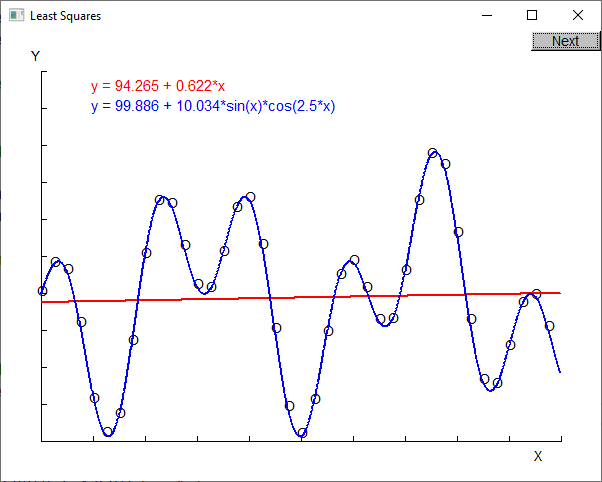
\includegraphics[width=0.6\textwidth]{images/least_squares_graphing.png}

    }
    \caption{Графическое представление данных}
\end{figure}

Вспомогательная функция \code{make\_regression()} создаёт лямбда-выражение, вычисляющее точки аппроксимирующей кривой. При~этом коэффициенты \(a\) и \(b\) скрыты в~реализации объекта лямбда-выражения:

\cppfile[firstline=26, lastline=29]{projects/ch15/least_squares/main.cpp}

Добавьте подпись кривой на~график "--- уравнение модели с~вычисленными коэффициентами. Далее, по аналогии добавьте модель с~нелинейной базисной функцией.



%%================
\WhatToReadSection
%%================
\textcite{Stroustrup:2016:ru}: \textbf{глава~16}



%%===============
\ExercisesSection
%%===============
\begin{exercise}
\item Выполните упражнения из \textbookref{главы~15} учебника.

\end{exercise}

%% !TEX encoding   = UTF8
% !TEX spellcheck = ru_RU
% !TEX root = ../seminars.tex

%%===============================================
\chapter{Графические пользовательские интерфейсы}
%%===============================================

%%====================================
\section{Окно с кнопкой \texttt{Quit}}
%%====================================
Выполним упражнение~1 из~\textbookref{главы~16} учебника. Для~этого пронаследуем \code{My\_window} от~класса \code{Simple\_window} из~библиотеки \code{Graph\_lib}. Затем добавим по~аналогии с~кнопкой \code{Next} кнопку \code{Quit}, как показано на~рисунке~\ref{fig:mywindow}.

\begin{figure}[ht]
    {\centering
        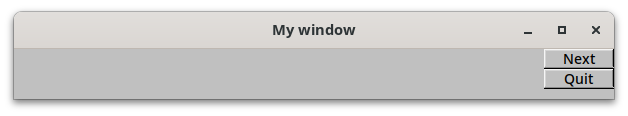
\includegraphics[width=0.6\textwidth]{images/my_window.png}

    }
    \caption{Простое окно \code{My\_window} с кнопкой \code{Quit}}
    \label{fig:mywindow}
\end{figure}

Из~документации к~библиотеке \name{FLTK} известно, что если все окна становятся скрытыми, то цикл обработки событий прекращает работу. То есть для~реализации функции \code{quit()} можно воспользоваться методом \code{hide()}.

\cppfile[firstline=11, lastline=21]{projects/ch16/chessboard/board.h}

Конструктор нашего окна принимает те же аргументы, что и \code{Simple\_window}. Мы добавляем инициализацию кнопки \code{Quit}. Нужно сместить её вниз на~высоту кнопки \code{Next}, которую добавляет базовый класс, а также связать её с~функцией-обработчиком \code{cb\_quit()}:

\cppfile[firstline=7, lastline=12]{projects/ch16/chessboard/board.cpp}

\textbf{NB!} Обратим внимание на одну деталь, которую нам пришлось изменить в~изначальной версии кода библиотеки \code{Graph\_lib}:

\cppfile[firstline=8, lastline=14]{projects/lib/Graph_lib/GUI.cpp}

\noindent В~строке~12 мы передаём указатель на~текущий объект класса (\code{this}), то есть указатель на~кнопку (\code{Button}), а не~указатель на~окно, как это ожидается в~примерах обработчиков, показаных в~\textbookref{главе~16} учебника.

Отметим, что здесь мы можем передавать, вообще говоря, любые данные. Позже библиотека \name{FLTK} вернёт нам указатель на~эти данные в~функцию обратного вызова:

\cppfile[firstline=14, lastline=18]{projects/ch16/chessboard/board.cpp}

\noindent Параметр \code{widget} как раз и есть тот самый адрес кнопки, который мы передаём при~вызове функции \code{Button::attach()}, когда связываем кнопку с~окном:

\cppfile[firstline=11, lastline=11]{projects/ch16/chessboard/board.cpp}

Оказывается, во многих задачах удобнее иметь указатель на~наш виджет. А, так как он хранит адрес окна, с~которым связан, мы можем получить доступ к~нашему окну и, в~конце концов, вызвать метод \code{quit()}:

\cppfile[firstline=17, lastline=17]{projects/ch16/chessboard/board.cpp}

\noindent Здесь использован оператор \code{dynamic\_cast}, который выполняет приведение типа от~ссылки на~объект базового класса к~ссылке на~объект производного класса (\textenglish{down cast}). Такое преобразование в~общем случае небезопасно. Данный оператор выполняет проверку во~время выполнения программы и возбуждает исключение \code{std::bad\_cast} в~случае ошибки.



%%=======================
\section{Шахматная доска}
%%=======================
Покажем, как можно создать клеточное поле и взаимодействовать с~ним на~примере упражнения~2 из~\textbookref{главы~16}. Эти идеи можно использовать для~создания практически любой игры с~клеточным полем: шашек, шахмат, сапёра, морского боя, пять в ряд и других.

Учитывая последующую доработку, код удобно сразу распределить между~несколькими файлами, как это предлагается в~таблице~\ref{tab:chessboard}.

\begin{table}[ht]
    {\centering\begin{tabular}{ll}
        \toprule
        \code{board.h}   & класс \code{Chessboard} для~шахматной доски, а также \code{My\_window} \\
        \code{board.cpp} & \\[0.5em]

        \code{cell.h}    & класс \code{Cell} для~шахматной клетки \\
        \code{cell.cpp}  & \\[0.5em]

        \code{main.cpp}  & \\
        \bottomrule
    \end{tabular}

    }
    \medskip
    \caption{Распределение кода <<шахматной доски>> между файлами}
    \label{tab:chessboard}
\end{table}

Размеры клеток и, соответственно, окна зафиксируем. Впоследствии, такое поведение можно изменить. Клетки представим квадратными кнопками и будем хранить их в~\code{Vector\_ref}. Метки строк и столбцов доски можно нарисовать при~помощи объектов \code{Marks}. Окно, согласно заданию, пронаследуем от~\code{My\_window} из~предыдущего упражнения.

\begin{figure}[ht]
    {\centering
        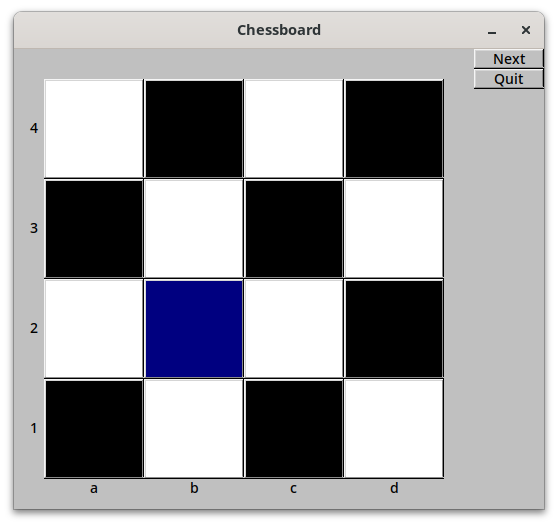
\includegraphics[width=0.5\textwidth]{images/chessboard.png}

    }
    \caption{Окно с шахматной доской \(4\times 4\)}
    \label{fig:chessboard}
\end{figure}

Итак, давайте разбираться по~порядку.



%%===========================
\paragraph{Шахматная клетка.}
%%===========================
Прежде всего, создадим шахматную клетку "--- класс \code{Cell}. Клетки на~шахматной доске могут быть только белыми или чёрными. Это свойство мы выразим, используя перечисление \code{Cell::Type}. Размер клетки зафиксируем на~этапе компиляции. Тогда разумно сделать его константой класса (\code{static}), чтобы обращаться из~любой точки программы без~указания объекта \code{Cell::size}.

Нам придётся перекрыть метод \code{attach()}. Почему?

Также добавим пару методов \code{activate()}/\code{deactivate()} для~управления подсветкой активной клетки (клетка~\code{b2} на~рисунке~\ref{fig:chessboard}), то есть той клетки, которую выбрал мышкой пользователь.

В~заголовочном файле \code{cell.h} разместим определение класса:

\cppfile[firstline=8, lastline=32]{projects/ch16/chessboard/cell.h}

Реализация методов проста и не~требует дополнительных пояснений, кроме того, что \code{pw} "--- это защищённый член класса \code{Graph\_lib::Widget}, связанный с~реальным графическим виджетом из~\name{FLTK}.

Код разместим в~файле \code{cell.cpp}:

\cppfile[firstline=5, lastline=32]{projects/ch16/chessboard/cell.cpp}



%%==========================
\paragraph{Шахматная доска.}
%%==========================
Основные моменты обозначены выше. Отметим здесь, что размер доски (\(N\times N\)) фиксируем на~этапе компиляции. Введём дополнительную константу \(N_{max}\), чтобы пользователь класса не~превышал определённый размер. Дело в~том, что позже мы будем добавлять подписи клеток и пока рассчитываем дизайн максимально на~8--9 клеток по~высоте. Дальше придётся что-то придумывать или каким-то образом выравнивать текстовые метки, состоящие из~двух цифр. (Это оставляем на~подумать.)

В~заголовочный файл \code{board.h} добавим определение класса:

\cppfile[firstline=23, lastline=51]{projects/ch16/chessboard/board.h}

Реализацию методов класса добавим в~файл \code{board.cpp}.

Конструктор задаёт размеры окна, создаёт клетки, располагая их в~соответствующих позициях, и рисует метки строк и столбцов доски. Зафиксируем размеры окна, чтобы пользователь не~смог его растягивать или сжимать. Сделать это позволяет функция \code{size\_range()} "--- метод окна \name{FLTK}.

\cppfile[firstline=48, lastline=67]{projects/ch16/chessboard/board.cpp}
\cpp/  .../
\cppfile[firstline=79, lastline=79]{projects/ch16/chessboard/board.cpp}

Цвет клетки (или тип) вычисляется на~основе номеров строки и столбца, определяющих её положение на~доске. Клетка в~левом нижнем углу имеет чёрный цвет. Обратим внимание, что клетки добавлялись в~линейный массив по~порядку в~соответствии с~направлением снизу вверх и слева направо, как принято в~шахматах.

\cppfile[firstline=20, lastline=26]{projects/ch16/chessboard/board.cpp}



%%=========================
\paragraph{Подписи клеток.}
%%=========================
Метки \code{Marks} допускают всего лишь один символ, поэтому мы используем ограничение \code{N\_max} для~максимального размера доски. Если потребуется вывести двузначные номера клеток, придётся разработать новый класс или добавить метки при~помощи неименованных объектов \code{Text}.

А пока воспользуемся простой реализацией (добавляем код в конструктор):

\cppfile[firstline=67, lastline=78]{projects/ch16/chessboard/board.cpp}

\noindent и парой внешних вспомогательных функций:

\cppfile[firstline=28, lastline=46]{projects/ch16/chessboard/board.cpp}

\noindent Таким образом, получается вид, как на~рисунке~\ref{fig:chessboard}.



%%=========================================
\paragraph{Взаимодействие с пользователем.}
%%=========================================
В~функцию-обработчик нажатия на~кнопку-клетку добавим простую логику самой шахматной доски. Можно:
\begin{itemize}
 \item выделить любую клетку;
 \item переместить выделение, выбрав другую клетку;
 \item снять выделение, нажав на~выделенную клетку повторно.
\end{itemize}

\noindent Реализация относительно проста, однако, здесь удобно использовать переменную-указатель \code{selected}. (Указатели будут обсуждаться в~\textbookref{главе~17} учебника.) Мы запоминаем адрес <<активной>> клетки в~переменной \code{selected}. Значение \code{nullptr} говорит, что <<активная>> клетка не~выбрана.

\cppfile[firstline=81, lastline=103]{projects/ch16/chessboard/board.cpp}

\noindent\textbf{NB!} Если в~отображении виджета что-то изменилось, то, скорее всего, потребуется перерисовать его вручную. Для~этого используйте \code{Fl::redraw()}.

Теперь настало время собрать и запустить программу целиком. Добавьте необходимые заголовки, функцию \code{main()}. Создайте окно \code{Chessboard} и запустите цикл обработки событий:

\cppfile[firstline=17, lastline=18]{projects/ch16/chessboard/main.cpp}



%%===============================
\section{Добавление фигур. Шашки}
%%===============================

\begin{figure}[ht]
    {\centering
        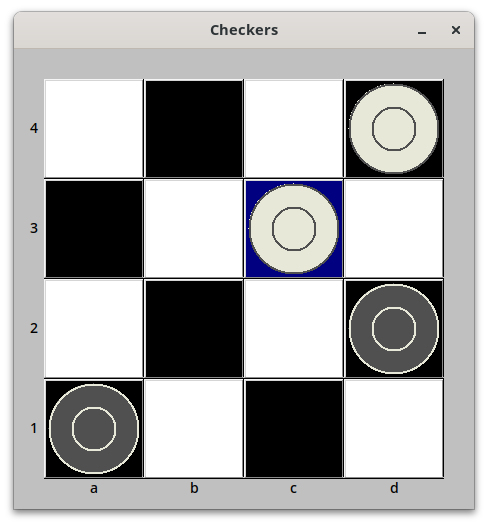
\includegraphics[width=0.5\textwidth]{images/checkers.png}

    }
    \caption{Шахматная доска \(4\times 4\) с~шашками}
    \label{fig:checkers}
\end{figure}

\todo{Описание будет добавлено позже.}



%%================
\WhatToReadSection
%%================
\textcite{Stroustrup:2016:ru}: \textbf{глава~17}



%%===============
\ExercisesSection
%%===============
\begin{exercise}
\item Выполните упражнения из~\textbookref{главы~16} учебника.

\end{exercise}

%\include{17/vector_and_free_store}
%\include{18/vectors_and_arrays}
%\include{19/vector_templates_and_exceptions}
%\include{20/containers_and_iterators}
%\include{21/algorithms_and_maps}
%\include{26/testing}


\backmatter
%%=========
\include{afterword}

\input{common/references}


\appendix
%========
\include{appendix}

\end{document}
